%%
% Please see https://bitbucket.org/rivanvx/beamer/wiki/Home for obtaining beamer.
%%
\documentclass[10pt]{beamer}

\renewcommand{\theenumi}{\alph{enumi}}
\usepackage{graphicx}

\title[Statistical Decision Theory]{Introduction to Decision Theory}

\author{Nishant D. Gurnani}
\date{July 4, 2020}


\begin{document}

% Title Page
\begin{frame}
\titlepage	
\end{frame}


% Big Picture
\begin{frame}
\frametitle{The Big Picture}
$$\text{financial markets} \rightarrow \text{data} \rightarrow \text{statistics} \rightarrow \text{inferences}$$
\newline 
As statisticians, we are tasked with turning the large amount of data generated by experiments and observations into inferences about the world.
\newline
\newline
This gives rise to a number of core statistical questions:
\newline

\begin{enumerate}

\item{Modeling: How do we capture the uncertainty in our data and the world that produced it?}
\newline
\item{Methodology: What are the right mathematical and computational tools that allow us to draw these statistical inferences?}
\newline
\item{Analysis: How do we compare and evaluate the statistical inferences we make and the procedures we use to make them? In particular, how do we do optimal inference?}	
\newline
\end{enumerate}

\end{frame}

% Framework 1
\begin{frame}
\frametitle{Decision Theory Framework}
Decision theory provides a framework to answer all of the core questions.
\newline
In particular, it allows us to formalize the notion of inference as a \textbf{decision problem} consisting of three key ingredients:
\newline
\begin{enumerate}
\item{A \textbf{statistical model} is a family of distributions $P$, indexed by a parameter $\theta$. We write $$ P = \{\mathbb{P}_{\theta} : \theta \in \Omega\}$$}

Here $\theta$ is the parameter, $\Omega$ is the parameter space, and each $\mathbb{P}_{\theta}$ is a distribution.\newline

$P$ is the class of distributions to which we believe our random sample $X$ belongs. In other words, we assume that the data $X$ come from some $\mathbb{P}_{\theta} \in P$ but that the true $\theta$ is unknown. \newline 

The fact that we don't know $\theta$ captures our uncertainty about the problem.    
 
\end{enumerate}
\end{frame}

% Framework 2
\begin{frame}
\frametitle{Decision Theory Framework}
\textbf{Example 1} (Weighted coin flips) \newline
\newline
Observe a sequence of coin flips $X_1,\dots,X_n \in \{0,1\}$ where 0 encodes tailes and 1 encodes heads. 
\newline
\newline
It's a weighted coin, so I don't know how often I expect heads to arrive. The goal is to estimate the probability of heads given the observations. 
\newline
\newline
To do this we model this process as independent draws from a Bernoulli distribution: $$P = \{\text{Ber}(\theta) : \theta \in [0,1] = \Omega \}$$
\newline
In this case, $\mathbb{P}_{\theta} (X_i = 1) = \theta$.

\end{frame}

% Framework 3
\begin{frame}
\frametitle{Decision Theory Framework}
\begin{enumerate}
\setcounter{enumi}{1}
\item{A \textbf{decision procedure} $\delta$ is a map from $\mathcal{X}$ (the sample space) to the decision space $\mathcal{D}$\newline
\newline
\textbf{Example 2} (Weighted coin flips)
\newline
\newline
Taking $P = \{\text{Ber}(\theta) : \theta \in [0,1] = \Omega \}$ as before, we may be interested in estimating $\theta$ or testing hypotheses based on $\theta$.
\newline
\begin{enumerate}[(a)]
\item{Estimating $\theta$: the decision space is $\mathcal{D} = [0,1]$, and the decision procedure might be $\delta(X) = \frac{1}{n} \sum^n_{i=1} X_i$. This procedure is an example of an \textbf{estimator}.}
\newline
\item{Accept or rejecting the hypothesis $\theta > 1/2$: the decision space is $\mathcal{D} = \{\text{accept}, \text{ reject}\}$, and one possible decision procedure is $\delta(X) = "\text{reject if} \frac{1}{n} \sum^n_{i=1} X_i \leq 1/2, \text{accept otherwise}"$ This procedure is an example of a \textbf{hypothesis test}.}
\end{enumerate}
}
\end{enumerate}
\end{frame}

% Framework 4
\begin{frame}
\frametitle{Decision Theory Framework}
\begin{enumerate}
\setcounter{enumi}{2}
\item{A \textbf{loss function} is a mapping $L: \Omega \times \mathcal{D} \rightarrow \mathbb{R}^{+}$. 
\newline
\newline 
$L(\theta, d)$ represents the penalty for making the decision $d$ when $\theta$ is in fact the true parameter for the distribution generating the data. 
\newline
\newline 
The goal is to assign penalties for bad decisions.
\newline
\newline 
\textbf{Example 3} (Squared-error loss). 
\newline
\newline 
For estimating a real-valued parameter $\theta$ with decision $d \in \mathbb{R} = \mathcal{D}$, a common loss function is the squared-error loss
$$ L(\theta, d) = (\theta - d)^2$$ 
}	
\end{enumerate}
	
\end{frame}



% Analyzing Procedures 1
\begin{frame}
\frametitle{Analyzing Procedures}
Decision theory is useful because it allows us to analyze statistical procedures.
\newline
\newline
The three components of a decision problem together give rise to our primary basis for evaluation - \textbf{the risk function}.

$$ R(\theta, \delta) = \mathbb{E}_{\theta}[L(\theta, \delta(X))] $$

The risk is $R(\theta, \delta)$ is the average loss incurred when the decision procedure $\delta$ is used over many draws of the data from its generating distribution $\mathbb{P}_{\theta}$.
\newline
\newline
The risk function gives us a way to compare and rule out procedures. 
\newline
\newline
$\delta$ is \textbf{inadmissible} if there exists $\delta'$ such that $R(\theta, \delta') \leq R(\theta, \delta)$ for all $\theta$ and  
$R(\theta', \delta') < R(\theta', \delta)$ for some $\theta'$.
\end{frame}

% Analyzing Procedures 2
\begin{frame}
\frametitle{Analyzing Procedures}
\textbf{Example 4} (Weighted coin flips)
\newline
\newline
For estimating the probability of heads $\theta$, let us consider three possible decision procedures:

\begin{enumerate}
\item{$\delta_{n}(X) = \frac{1}{n} \sum_{i=1}^n X_i$ be the sample mean of the first n data points}

\item{$\delta_1(X)$ = naive estimator that uses the outcome of just one flip}

\item{$\delta_{\text{goofy}}(X) = \frac{1}{2}$ which is a fixed constant}	

\end{enumerate}

\vspace{10pt}
Under the loss function $L(\theta, d) = (\theta - d)^2$ the risk of each is:

\begin{enumerate}

\item{$R(\theta, \delta_n) = \mathbb{E}_{\theta}[(\theta - \delta_n(X))^2] = \frac{\theta(1-\theta)}{n}$}

\item{$R(\theta, \delta_1) = \mathbb{E}_{\theta}[(\theta - \delta_1(X))^2] = \theta(1-\theta)$}

\item{$R(\theta, \delta_{\text{goofy}}) = (\theta - \frac{1}{2})^2$}

\end{enumerate}
\vspace{10pt}
Which one is the best procedure?
\end{frame}

% Analyzing Procedures 3
\begin{frame}
\frametitle{Analyzing Procedures}
Clearly there is no uniformly best procedure, to develop concrete notions of optimality we must induce an optimizable problem.
\begin{figure}
	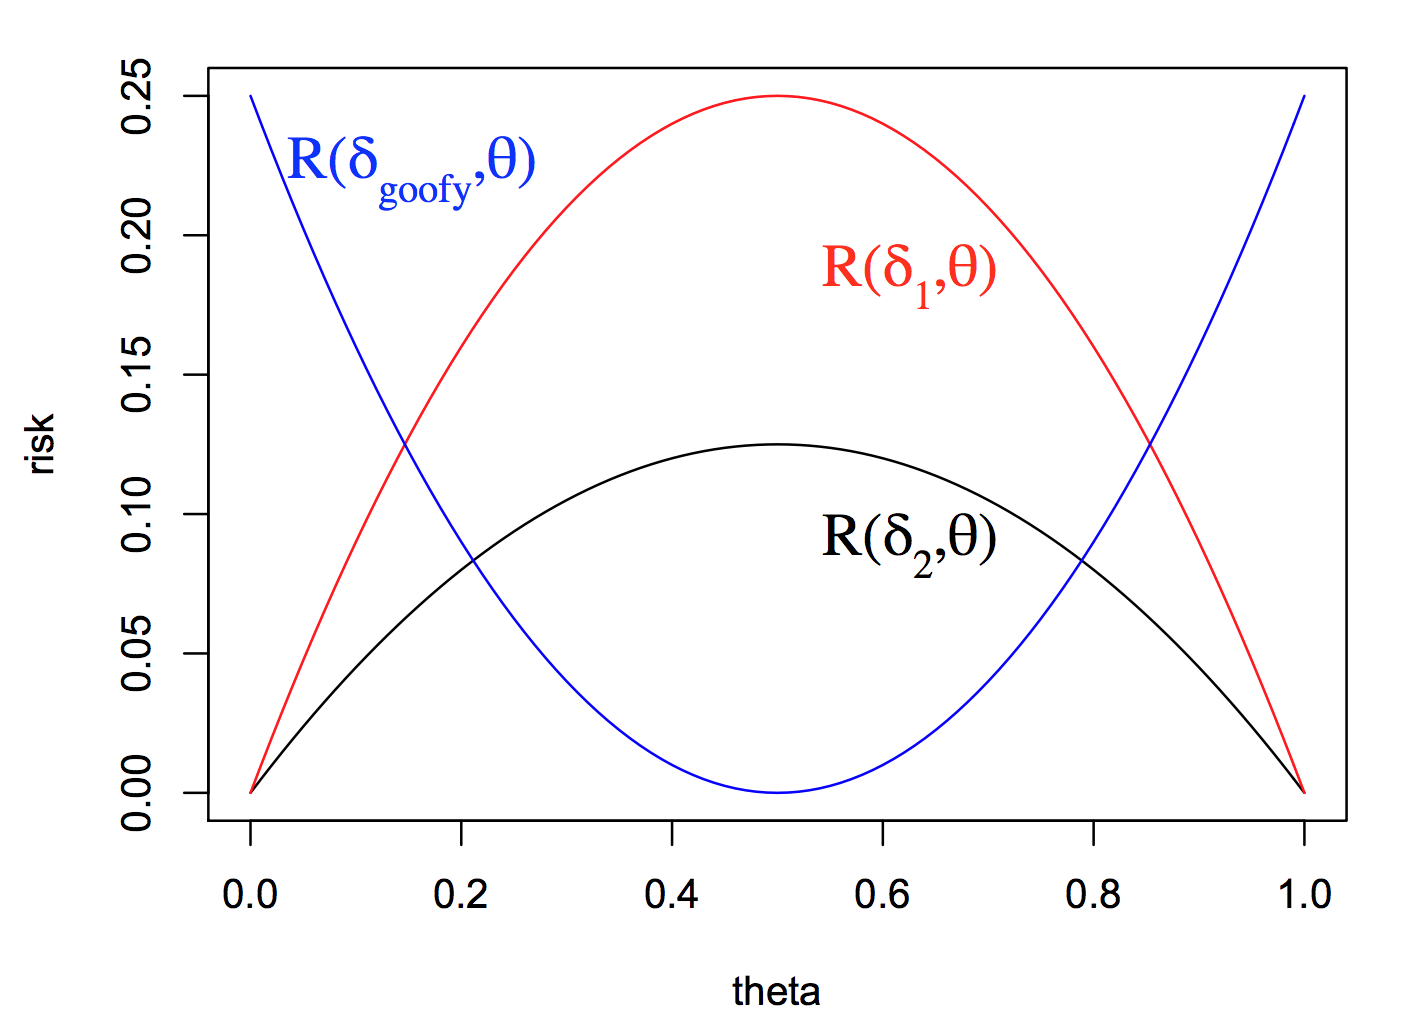
\includegraphics[width=0.8\textwidth]{risk.png}
\end{figure}
\end{frame}


% Analyzing Procedures 4
\begin{frame}
\frametitle{Optimal Inference}
To develop our theory of optimality we change the requirements of our decision problem. 
\newline
\newline
In particular, we try to induce an optimizable problem by taking one of the following actions:
\newline

\begin{enumerate}
\item{
\textbf{Constrain} the set of decision procedures under consideration, by requiring our procedures to satisfy criteria like unbiasedness or invariance.
\newline
\begin{enumerate}[(a)]
\item{Unbiased estimators: we say that $\delta$ is unbiased for estimating $g(\theta)$ if $\mathbb{E}_{\theta}[\delta(X)] = g(\theta)$}
\newline
\item{Equivariance or invariance: enforce symmetries in the decision procedure. For example, location invariance requires an estimator to satisfy $\delta(X + c) = \delta(X) + c$}
\end{enumerate}
}	
\end{enumerate}	
\end{frame}

% Analyzing Procedures 5
\begin{frame}
\frametitle{Optimal Inference}
\begin{enumerate}
	
\setcounter{enumi}{1}

\item{
\textbf{Collapse} the risk function into a single numerical summary and minimize this overall summary of risk instead of requiring uniformly lower risk.
\newline
\begin{enumerate}[(a)]
\item{Bayes procedures minimize the average risk $\int R(\theta, \delta)d\Lambda(\theta)$ where $\Lambda$ is a probability distribution (the prior distribution) over $\Omega$.}
\newline
\item{Minimax procedures minimize the worst-case risk, $\sup_{\theta \in \Omega} R(\theta, \delta)$, and hence achieve the best worst-case performance.}
\end{enumerate}
}	
\end{enumerate}
\vspace{10pt}
These principles are foundational to the theory of optimal inference and apply both in the context of point estimation and hypothesis testing.
\end{frame}

\end{document}
